\chapter{\label{chap:intro}Introdução}

Em 2014, 54\% da população mundial vivia em áreas urbanas, de acordo com a Organização das Nações Unidas~\cite{UN14}. A expectativa é que esta proporção aumente para 66\% até o ano 2050. Em números absolutos isto representa um acréscimo de 2,5 bilhões de pessoas à população urbana mundial nos próximos 35 anos. Uma das consequências da alta densidade populacional em regiões geográficas limitadas é o crescimento do modelo de verticalização na construção civil. Neste cenário, onde prédios de diversos andares se tornam presença no cotidiano da maioria da população, os elevadores passam a um papel de destaque.

Uma pesquisa realizada pela IBM no ano de 2010 em 16 cidades norte-americanas constatou que, durante 12 meses, o tempo acumulado no qual trabalhadores de escritórios\footnote{Em uma força de trabalho total de 51 milhões de trabalhadores, dos quais 12,7 milhões são usuários de elevadores diariamente~\cite{IBM10}.} aguardaram por elevadores foi de 92 anos~\cite{IBM10}. Em uma economia onde o salário horário médio de um trabalhador é de US\$ 24,99, o tempo de espera por elevadores representa custos de mais de US\$ 20 bilhões em média por ano~\cite{BLS15}.

Além do impacto econômico existe o impacto psicológico. Trabalhadores em centros metropolitanos empreendem uma parcela significativa da sua rotina no deslocamento entre residência e local de trabalho e no caminho inverso ao final do dia. Além de gastar uma quantidade significativa de tempo no trânsito das ruas, em carros, ônibus, bicicletas e metrôs, o tempo compreendido entre aguardar o elevador e desembarcar no andar desejado está longe de ser desprezível. Em função disso, ajustam sua rotina abrindo mão de momentos de momentos de descanso ou lazer. Uma possível consequência é um aumento nos níveis de estresse e um decréscimo na qualidade de vida a médio e longo prazo. {\color{red}[BUSCAR FONTES PARA ESTE PARÁGRAFO]} % TODO: CITATIONNEEDED

\begin{figure}[htb!]
\centering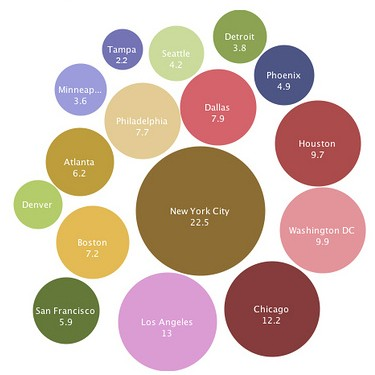
\includegraphics{img/time-cost.jpg}
\caption{\label{fig:fig1}Tempo de espera acumulado (em anos) por elevadores durante 12 meses em 16 cidades norte-americanas. Fonte:~\cite{IBM10}}
\end{figure}

Neste contexto global, a indústria de elevadores possui alguns desafios: primeiro, lidar com a pressão para a redução de custos na construção civil, construindo elevadores mais baratos e eficientes, com melhorias no desempenho de transporte; segundo, competir no mercado oferecendo serviços novos, personalizados e com garantia de qualidade, visando revolucionar a maneira com que elevadores interagem e servem passageiros~\cite{KOEHLEROTTIGER02}. Já sob o ponto de vista dos passageiros, estes esperam que suas chamadas sejam atendidas imediatamente e que sejam levados ao seu destino o mais rápido possível.

Existem diversas abordagens que os fabricantes de elevadores podem usar para minimizar o tempo de espera, como aumentar o número de elevadores no prédio ou a capacidade de cada elevador. Entretanto, este tipo de alteração não é sempre realizável em função de limitações na estrutura do prédio ou inviabilidade financeira. Como alternativa e muitas vezes uma solução de mais fácil aplicação é otimizar o sistema de controle dos elevadores. Ainda assim, a tarefa de atribuir elevadores para atender chamadas minimizando o tempo médio de espera está no conjunto de problemas NP-difícil (ou NP-hard, ou NP-complexo)~\cite{SeKo99}. Portanto, uma solução ótima para este problema ainda não é conhecida.

Desde meados dos anos 1980, a indústria de elevadores vem estudando e implementando estratégias para encontrar soluções sub-ótimas para o problema. Diversas técnicas de Inteligência Artificial foram adotadas, como redes neurais, algoritmos genéticos, lógicas \textit{fuzzy} e, mais recentemente, sistemas multi-agentes, planejamento e aprendizado de máquina~\cite{KOEHLEROTTIGER02}.

A proposta deste trabalho é construir um simulador de elevadores e utilizá-lo para comparar diferentes estratégias de controle em diferentes cenários. O usuário do simulador poderá:

\begin{itemize}
  \item Definir cenários (número de andares; número de elevadores; população do prédio; distribuição de chegada de passageiros; etc);
  \item Selecionar um algoritmo para controle dos elevadores ou implementar o seu próprio;
  \item Comparar o desempenho entre diferentes algoritmos em um mesmo cenário;
  \item Comparar o desempenho de um algoritmo em múltiplos cenários.
\end{itemize}

Espera-se que com os resultados das simulações seja possível avaliar quais estratégias são viáveis em quais cenários e, em última análise, sugerir uma estratégia superior às demais.

\section{Motivação prática}

\section{Glossário}

Termos chaves usados neste trabalho.

\begin{description}[leftmargin=!,labelwidth=\widthof{\bfseries Sistema de Controle}]
  \item[Lobby]                Andar térreo de um prédio.
  \item[Elevador]             Dispositivo de transporte vertical que movimenta pessoas ou cargas entre andares ou níveis de um prédio ou estrutura.
  \item[Sistema de Controle]  O sistema central que gerencia todos os elevadores.
\end{description}